% !TEX root =  ../main.tex
\section{Overview}
\label{overview}


Figure~\ref{fig:framework} illustrates our workflow.
\Pa and \Pb are addressed sequentially: From a given problem (a) we first plan a root guide path (b), before
extending it into a sequence of static equilibrium configurations(c). In the case where step c fails,
our framework invalidates the computed guide path, and restarts the planning from b.

%

\subsection{Computation of a guide path --- \Pa (Section~\ref{rbprm})}
We first consider the problem of planning a root guide path (Figure~\ref{fig:framework}--$\mathcal{P}_1$).  The dimension of the path is equal to the number of degrees of freedom (DoFs) of the root of the robot.
Similarly to previous work~\citep{Bouyarmane2009} the path must be \textit{equilibrium feasible}: there must exist a joint configuration that results in static equilibrium for each root configuration\footnote{Enforcing static equilibrium is a classical, conservative approach to reduce the search space and considering states  with non-zero accelerations and velocities, which can't be connected trivially. This does not mean that the final motion will necessary be quasi-static.}. Previous works verifiy \textit{equilibrium feasibility} by explicitly computing such a configuration. We preserve the low dimensionality of the problem by approximating \textit{equilibrium feasibility} with \textit{contact rechability}, illustrated in the following.

An intuitive description of \gls{contact reachable} configurations is ``close, but not too close'' to the environment: close, because a contact surface must be partially included in the reachable workspace of the robot to allow contact creation; not too close, because the robot must avoid collision.
%~ \deladp{\textit{Contact reachability} is verified with the \textit{reachability condition}, a geometrical criterion based on this intuitive description (Figure~\ref{fig:reach_cond}).}
More precisely, a root configuration is \textit{contact reachable} if the root scaled by a user-defined factor $s \geq 1$ is not in collision (Figure~\ref{fig:reach_cond} - red shape), while the reachable workspace is in collision (Figure~\ref{fig:reach_cond} - green shapes).
%~ Verifying the \textit{reachability condition} is very efficient in practice.
To plan a root path, we then use an RRT planner where, instead of checking collision to validate a configuration, we verify the \textit{reachability condition}.
%~ In Section~\ref{rbprm} we detail how  we define and use the \textit{reachability condition} to compute a guide path with the Reachability-Based RRT (Figure~\ref{fig:framework}---\Pa).

\begin{figure}[t]
\centering
  \begin{overpic}[width=0.8\linewidth]{figures/reachability_cond}
	\end{overpic}
\caption{The reachability condition is verified by the right configuration: the trunk (red) is free of collisions while the limbs reachable workspace (green) intersect the environment.}
		   \label{fig:reach_cond}
\end{figure}



%
%~ Ideally we would like to sample root configurations that are \gls{equilibrium feasible}. A root configuration is \gls{equilibrium feasible} if and only if there exists at least one joint configuration such that:
%~ \begin{description}
%~ \item[C1]: the robot is not in collision with the environment, 
%~ \item[C2]: the robot is in static equilibrium. 
%~ \end{description}
%~ Verifying C2 is computationally expensive because it requires the projection of the whole-body configuration into a contact posture, as well as the resolution of a linear program to compute the contact forces~\citep{Prete2016}.
%~ For this reason, we are interested in finding an approximation of the \glslink{equilibrium feasible}{\textit{equilibrium feasibility}} that is computationally efficient.
%~ A requirement for C2 is the condition:
%~ \begin{description}
%~ \item[C3]: at least one end-effector is in contact with the environment.
%~ \end{description}
%~ C1 and C3 define \glslink{contact reachable}{\textit{contact reachability}}, which is easier to verify than \glslink{equilibrium feasible}{\textit{equilibrium feasibility}} because it does not require the computation of contact forces.
%~ We make the assumption that for the \textit{\gls{cluttered} contact planning problem}, most of the times \gls{contact reachable} root configurations are also \gls{equilibrium feasible}.
%~ For this reason we neglect C2 during the resolution of $\mathcal{P}_1$, and we consider it only when solving \Pb.
%~ However, even verifying \glslink{contact reachable}{\textit{contact reachability}} is computationally too expensive because it requires the projection of the whole-body configuration into a contact posture.
%~ 
%~ An intuitive description of \gls{contact reachable} configurations is ``close, but not too close'': close, because a contact surface must be partially included in the reachable workspace of the robot (represented for the right leg in Figure~\ref{fig:contact_gen}--a); not too close, because the robot must avoid collision.
%~ We approximate \glslink{contact reachable}{\textit{contact reachability}} with the \textit{reachability condition}, a geometrical criterion based on this intuitive description.
%~ More precisely, a root configuration is \textit{reachable} if the root scaled by a factor $s \geq 1$ is not in collision, while the reachable workspace is in collision with the environment.
%~ Verifying the \textit{reachability condition} is very efficient in practice.
%~ In Section~\ref{rbprm} we detail how  we define and use the \textit{reachability condition} to compute a guide path with the Reachability-Based RRT (Figure~\ref{fig:framework}---\Pa).

In the remainder of this paper, we use the terms \gls{contact reachable} and \gls{equilibrium feasible} to qualify either a root or a whole-body configuration, or a set
of such configurations.


\subsection{Generating a discrete sequence of contact configurations --- \Pb (Section~\ref{sec:contact})}
The second stage extends the guide path into a sequence of contact configurations (Figure~\ref{fig:framework}--$\mathcal{P}_2$).
To achieve this the root path is first decomposed into a sequence of discrete root configurations, according to a user-defined discretization step.
Each root configuration is then extended into a whole-body configuration in static equilibrium.
The algorithm thus proceeds iteratively, starting from the whole-body initial configuration of the robot.
It takes advantage of the fact that each root configuration is fixed to generate the contact by considering each limb individually. 
%~ Candidate limb configurations resulting in the end-effector being close to the environment are selected from a database computed offline independently from the environment).
%~ Then we select one of these configurations based on user-defined heuristics (Figure~\ref{fig:contact_gen}), detailed in Appendix~\ref{sec:heuristics}.

%~ The details of the contact sequence generation are given in Section~\ref{sec:contact}. 

%~ From a given start configuration, the planner proceeds in an iterative fashion along the discretized path: given a new root configuration, an inverse-kinematics solver 
%~ is used to maintain the contacts that were previously existing. Possibly, some of these contacts cannot be maintained (because of joint limits or collisions).
%~ Then the contacts are broken. Conversely, new contacts are created to ensure the static equilibrium of the robot.
%~ The algorithm is designed so that only one contact can be created or broken between two successive configurations. While it does not provide guarantees that the interpolation between two configurations is achievable, it appears empirically as a reasonable heuristic.


%~ To create a contact, we consider each limb of the robot as a manipulator arm attached to the root. We store a database of configurations for each manipulator. Figure~\ref{fig:contact_gen} -- 2 presents a few configurations for the right arm of the robot. The configurations in the database which are close to contact are considered (Figure~\ref{fig:contact_gen} -- 2 and 3). Among the candidates, 3 criteria are considered to choose the most relevant: the ideal candidate is free of collision, allows to maintain static balance if necessary, and  contributes to the motion in an optimal way. We call the measure of this contribution task efficiency: it represents the ability the limb has to exert a force compatible with the direction of motion. In Figure~\ref{fig:contact_gen} -- 4, the black arrow represents the direction of motion. Among the candidates, the most relevant to achieve a vertical motion is chosen, and projected on the contact surface using an inverse kinematics solver (Figure~\ref{fig:contact_gen} -- 5). The task efficiency is measured using the Extended FORce Transmission ratio (EFORT), proposed by ~\cite{Tonneau:2014:TEC:2619648.2619652}.



\section{Notation and definitions} \label{notations}

A vector  $\mathbf{x}$ is denoted with a bold lower-case letter.
A matrix $\mathbf{A}$ is denoted with a bold upper-case letter.
A set $C$ is denoted with an upper-case italic letter.
Scalar variables and functions are denoted with lower-case italic letters, such as
$r$ or $f(\textbf{x})$.

%\subsubsection{Robot description}
%\label{def}

%~ \begin{figure}
  %~ \centering
  %~ \begin{overpic}[width=0.8\linewidth]{figures/character}
    %~ \put (7,29) {\small{$\in \mathbf{q}^1$}}
    %~ \put (7,25) {\small{effector}}
  %~ \end{overpic}
  %~ \caption{
    %~ Left: Robot in a rest configuration. The right arm is denoted as the limb $R^1$. Each colored dot represents a degree of freedom around an axis. Right: Volumes of the robot. The red geometry denotes $W^0$ and must remain collision-free. The green spheres are the reachable workspace of each limb, the  $W^k$.}
  %~ \label{fig:character}
%~ \end{figure}


\medskip
\textbf{A robot} is a kinematic tree $R$ composed of: a root $R^0$, and $l$ limbs $R^k, 1 \leq k \leq l$, attached to the root.
The root has $r \geq 6$ DoFs: for instance, HRP-2 has two extra DoFs in the torso, such that we have $r=8$.
Thus $R$ is fully described by a configuration (a vector of joint values) $\mathbf{q} \in  \mathbb{R}^{r+n}$, with $n$ the number of joint DoFs.
$\mathbf{q}$ is decomposed as follows:
\begin{itemize}
	\item $\mathbf{q}^k$ is a configuration  of the limb $R^k$; % (Figure~\ref{fig:character});
	\item $\mathbf{q}^{\overline{k}}$ is a vector of joint values of R \textbf{not} related to $R^k$. We define for convenience \mbox{$\mathbf{q}= \mathbf{q}^k \oplus \mathbf{q}^{\overline{k}}$}; %Abusively, we denote by $\mathbf{q}^0 \oplus \mathbf{q}^k$ any configuration respecting $\mathbf{q}^0$ and $\mathbf{q}^k$;
	\item $\mathbf{q}^{0}\in \mathbb{R}^r$ is the world coordinates vector of $R^0$.
\end{itemize}
%Finally, $ \mathbf{q}_{start}$ and  $\mathbf{q}_{goal}$ are the start and goal configurations given as an input of our problem.

%\subsubsection{Environment and other volumes} 
%\label{sec:A}
\medskip
We then define a set of 3d volumes  $W^i, 0 \leq i \leq l$, each  attached to one joint of the root, such that 
$W^i(\mathbf{q}^{0})$ describes the world position of $W^i$ for the root configuration $\mathbf{q}^{0}$.

\noindent $W^0$ is a volume encompassing $R^0$ (Figure~\ref{fig:HyQ_roms}), or equal to it\footnote{$W^0$ is typically a low-polygonal bounding shape
of $R^0$ for performance.}.\\
 %~ (Figure~\ref{fig:character}-right: central cylinder). 
 $W^k$ is the reachable workspace of a limb $R^k$: %(Figure~\ref{fig:character}-right: the four ellipses). 
\begin{equation}
  W^k = \left\{ {\mathbf{x} \in \mathbb{R}^3: \exists \, \mathbf{q}^k \in C^k_{j.lim}, \mathbf{p}^k(\mathbf{q}^k) = \mathbf{x} } \right\}
\end{equation}
%~ \adnote{in this definition you don't account for joint limits}
where $\mathbf{p}^k$ denotes the end-effector position (in the root frame) of $R^k$ (translation only) for $\mathbf{q}^0 = \mathbf{0}$ being the null displacement, and  $C^k_{j.lim}$ is the space
of admissible limb joint configurations. We also define \mbox{$W = \bigcup_{k=1}^{l}W^k$}. 

%~ Each $W^i, 0 \leq i \leq l$ is  attached to one joint of the root, such that 
%~ $W^i(\mathbf{q}^{0})$ is the volume $W^i$ transformed the by root configuration $\mathbf{q}^{0}$.

\medskip
\textbf{The environment} $O$ is defined as the union of the obstacles $O_i$ that it contains.

\medskip
Finally we define some relevant subsets of the configuration space $C$.
$C_{Contact}$ is the set of whole body-configurations in contact and collision-free.
$C_{Contact}^k \subset C_{Contact}$ is the set of whole body-configurations where at least $R^k$ is in contact.

\medskip
$C_{Equil} \subset C_{Contact}$ is the set of whole body-configurations in static equilibrium and collision-free.

\medskip
For any set $C_{X}$, we define $C_{X}^0$:
\begin{equation*}
  C_{X}^0 = \left\{ \mathbf{q}^{0},  \exists \mathbf{q}^{\overline{0}}: \mathbf{q}^0  \oplus \mathbf{q}^{\overline{0}} \in C_{X} \right\}
\end{equation*}

%~ Finally, we define $dist(\mathbf{x}, O)$ as the minimal distance between a point $\mathbf{x}$ and the closest surface of the environment.
\begin{figure}
  \centering
  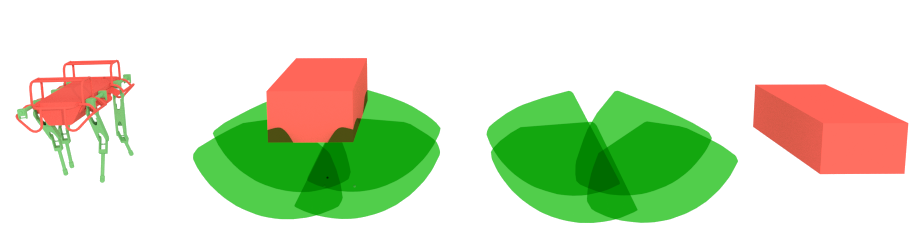
\includegraphics[width=0.95\linewidth]{figures/HyQ_roms}
  \caption{
           Reachable workspace and torso bounding box of HyQ. Each green shape represent a reachable workspace $W^k$ of a limb. The red shape is $W^0$.}
		   \label{fig:HyQ_roms}
\end{figure}
